\documentclass[conference]{IEEEtran}
\IEEEoverridecommandlockouts
% The preceding line is only needed to identify funding in the first footnote. If that is unneeded, please comment it out.
\usepackage{cite}
\usepackage{amsmath, amssymb, amstext, amsfonts, mathrsfs}
\usepackage{algorithmic}
\usepackage{graphicx}
\usepackage{textcomp}
\usepackage{xcolor}
\usepackage{hyperref}
\usepackage{amsmath}

\def\BibTeX{{\rm B\kern-.05em{\sc i\kern-.025em b}\kern-.08em
    T\kern-.1667em\lower.7ex\hbox{E}\kern-.125emX}}
    
% Kopf- und Fußzeile bearbeitbar machen
\usepackage{fancyhdr}
% Nun gestalten wir die Kopf-und Fußzeile
\pagestyle{fancy}
\rhead{\today}
\lfoot{Mader Mendes Marco \\ Späth Marco \\ Walker Dustin \\}
\cfoot{\thepage}
\rfoot{Signale und Systeme 2 \\ Dr. Prof. Haslach}
\renewcommand{\headrulewidth}{0pt}
\renewcommand{\footrulewidth}{0.4pt}
 
\begin{document}


\title{Signale und Systeme 2 - Praktikum: Abgabe 1}

\author{\IEEEauthorblockN{Mader Mendes Marco}
\IEEEauthorblockA{
\textit{Matrikelnummer: 763153}} % \\
%email address}
\and
\IEEEauthorblockN{Späth Marco}
\IEEEauthorblockA{\textit{Matrikelnummer: 763174}} % \\
%email address}
\and
\IEEEauthorblockN{Walker Dustin}
\IEEEauthorblockA{\textit{Matrikelnummer: 763190}} %//
% matthias.rauscher@student.reutlingen-university.de}
}

\maketitle
\newpage
\pagebreak
\vspace{30cm}


\newpage
\pagebreak
\vspace{30cm}

\newpage
\newpage
\newpage
\pagebreak
\vspace{30cm}
\section{Aufgabe 1}
\subsection{Anzahl der benötigten Mikrofonzahl}
\subsubsection{Auswertung mit einem Mikrofonen}
Ein Mikrofon könnte nur den Abstand \textit{r} der Schallquelle zum Mikrofon erkennen. Damit ist keine Positionserkennung möglich, da alle Punkte mit Abstand \textit{r} infrage kommen. 
Alle diese möglichen Punkte bilden eine Kugeloberfläche um den Mittelpunkt (die Position des Mikrofons), mit dem Abstand \textit{r}.

\subsubsection{Auswertung mit zwei Mikrofonen}
Mit zwei Mikrofonen ist eine Eingrenzung der möglichen Positionen der Schallquelle möglich, da nur noch die Schnittmenge der beiden Kugeloberflächen um die Mikrofone als Positionen in Frage kommen. Diese Schnittmenge stellt einen zweidimensionalen Kreisumfang dar. Siehe Abbildung \ref{fig:Normalfall beim Schnitt zweier Kugeloberflächen}. Dieser besteht aber immer noch aus $\infty$ Punkten und ist deshalb im Normalfall nicht geeignet zur Positionsbestimmung. Nur für den Sonderfall, dass die Schallquelle exakt im Mittelpunkt der Geraden zwischen Mikrofon 1 und 2 liegt kann die Position eindeutig bestimmt werden. Siehe Abbildung \ref{fig:Sonderfall beim Schnitt zweier Kugeloberflächen}.
\begin{figure}[b]
	\centering
	\begin{minipage}[t]{0.45\linewidth}
		\centering
		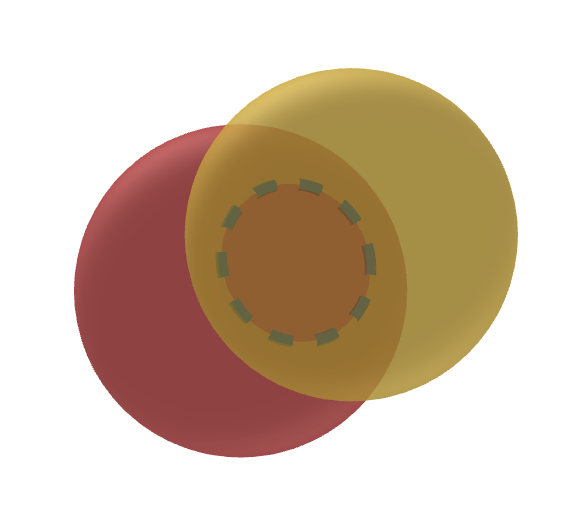
\includegraphics[width=0.75\textwidth]{Schnitt_2_Kugeln}
		\caption{Normalfall beim Schnitt zweier Kugeloberflächen}\label{fig:Normalfall beim Schnitt zweier Kugeloberflächen}		
	\end{minipage}
	\hfill
	\begin{minipage}[t]{0.45\linewidth}
		\centering
		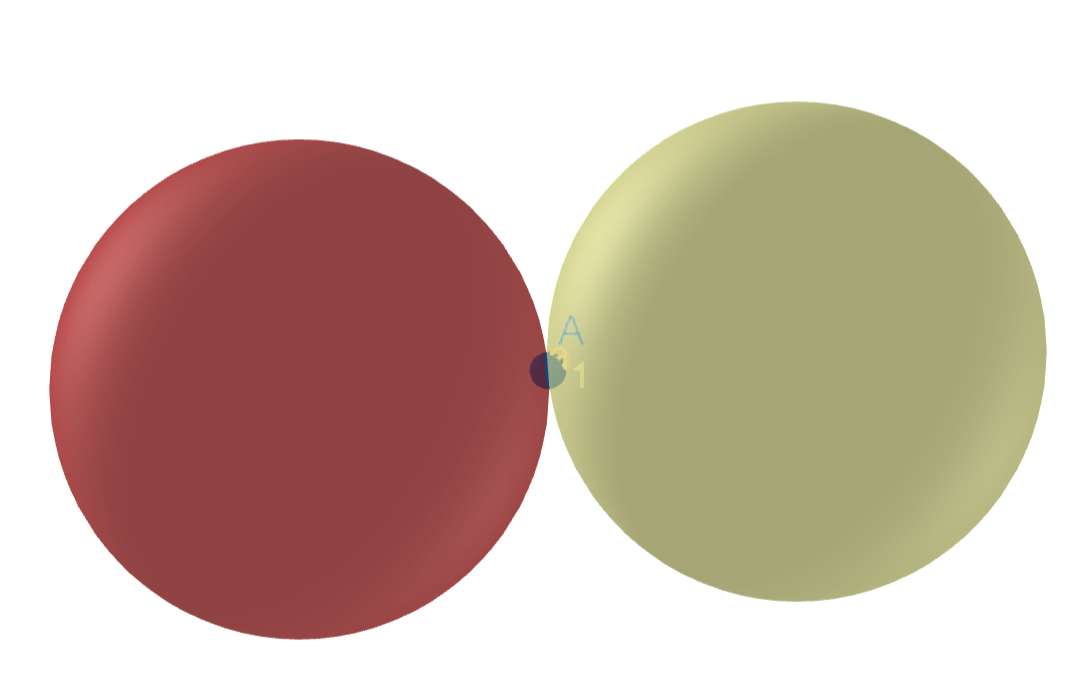
\includegraphics[width=0.75\textwidth]{2KugelnSonderfall}
		\caption{Sonderfall beim Schnitt zweier Kugeloberflächen}\label{fig:Sonderfall beim Schnitt zweier Kugeloberflächen}
	\end{minipage}
\end{figure}

\subsubsection{Auswertung mit drei Mikrofonen}

Durch die Detektion der Schallquelle mit drei Mikrofonen ist die Eingrenzung der möglichen Orte der Schallquelle auf zwei Punkte möglich. Die Orte der drei Schallquellen bilden immer eine Ebene im Raum, es ist nicht möglich, dass sich nur zwei in einer Ebene befinden und das Dritte außerhalb liegt. Darin liegt auch das Problem der zwei Punkte. Einer der beiden Punkte liegt oberhalb der Ebene aus den Mikrofonen mit einem Abstand $\lambda$ zur Ebene. Der Zweite liegt auf einer Geraden, die durch den ersten möglichen Punkt verläuft und orthogonal zur Mikrofonebene ist. Er hat den Abstand -$\lambda$ zur Ebene. Siehe Abbildung \ref{fig:Schnittpunkte dreier Kugeloberflächen}.
Bei der Aufgabenstellung soll ein Raum mit 1m x 1m x 1m Größe nach der Schallquelle durchsucht werden. Wenn die Mikrofonebene in einer der Begrenzungsebenen des Versuchsraums liegt, reichen 3 Mikrofone aus, da der andere Schnittpunkt der möglichen Orte der Schallquelle damit außerhalb des Versuchsraums liegt. Wenn die Mikrofonebene keine der Raumbegrenzungsebenen darstellt, sind drei Mikrofone nicht ausreichend. 
\begin{figure}
\centering 
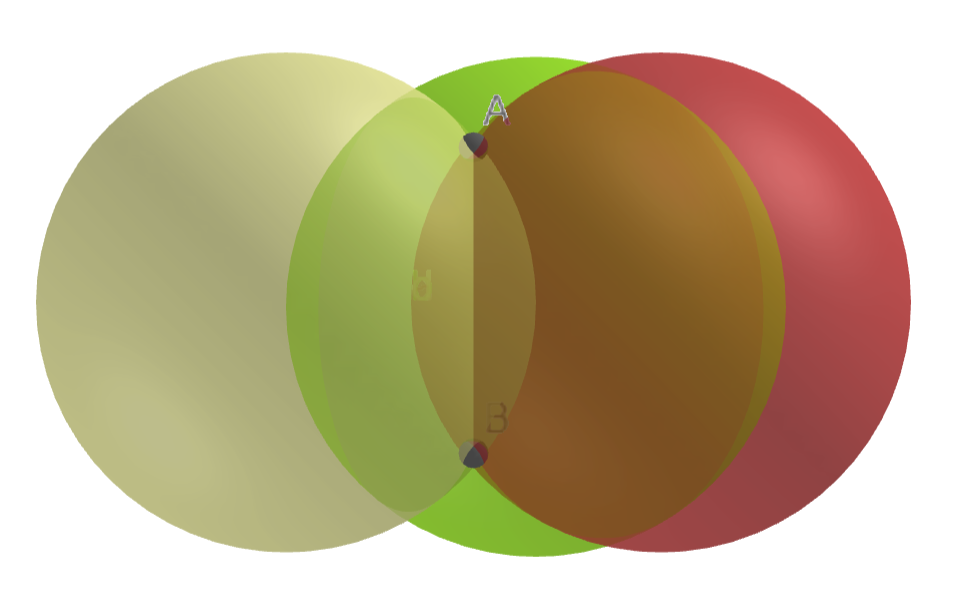
\includegraphics[width=0.4\textwidth]{3Kugeln}
\caption{Schnittpunkte dreier Kugeloberflächen}\label{fig:Schnittpunkte dreier Kugeloberflächen}
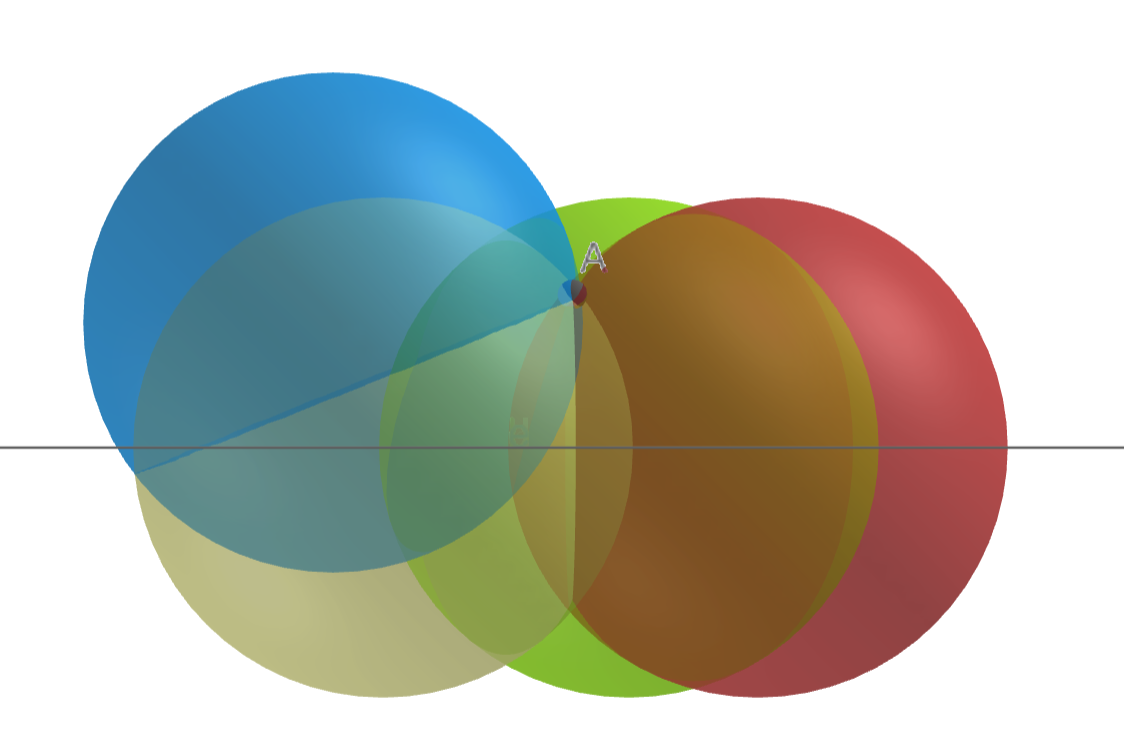
\includegraphics[width=0.4\textwidth]{4Kugeln}
\caption{Eindeutige Schnittpunktbestimmung durch vier Kugeloberflächen}\label{fig:Eindeutige Schnittpunktbestimmung durch vier Kugeloberflächen}
\end{figure}
\subsubsection{Auswertung mit 4 Mikrofonen}
In unserem Fall haben wir nicht die absolute Distanz, zwischen Schallquelle und Mikrofon, sondern nur die Laufzeitunterschiede zwischen den einzelnen Mikrofonen.Im dreidimensionalen Raum benötigen wir drei Informationen. Um drei Laufzeitdifferenzen zu erhalten, benötigen wir vier Mikrofone. 

Wenn sich das vierte Mikrofon nicht in einer Ebene mit den anderen dreien befindet, kann dadurch die Eindeutigkeit des Schnittpunktes zeitgleich garantiert werden. Da damit einer der beiden Schnittpunkte aus dem Fall mit drei Mikrofonen wegfällt. Siehe Abbildung \ref{fig:Eindeutige Schnittpunktbestimmung durch vier Kugeloberflächen}. Für unser Newtonverfahren müssen wir also mit vier Mikrofonen den Versuch aufbauen.



%______________________________________________________________________________________________
\newpage
\pagebreak
\section{Aufgabe 2}
\subsection{Mathematischer Ansatz: Newtonverfahren}
Aus den Zeitverschiebungen, mit der das Signal der Schallquelle von den Mikrofonen aufgenommen wird, kann die Position der Schallquelle im Raum näherungsweise bestimmt werden. Für das Newtonverfahren muss ein erster Ort der Schallquelle geschätzt werden, von welchem aus in mehreren Iterationen der reale Ort der Schallquelle immer besser angenähert werden kann. In einigen Fällen kommt das Newtonverfahren aber zu keinem korrekten Ergebnis. Das ist abhängig von der Positionierung der Mikrofone im Raum, dem Ort der Schallquelle, sowie der Schätzung der ersten Position des Objekts. 

Die Zeitverschiebung der Signale kann durch die Korrelation der Signale S1,S2 und S3 gegen das Signal S0 berechnet werden. Im Buch "Mathematik der digitalen Medien" von Bossert und Bossert wird das Verfahren für den zweidimensionalen Raum sehr ausführlich beschrieben. Weitere Erklärungen zum Verfahren können dort im Kapitel 2.3 unter "zweidimensionale Positionsbestimmung" nachgelesen werden. Auf dieser Arbeit beruhen unsere Berechnungen. Das Verfahren kann sehr leicht auf die hier benötigte, dritte Dimension erweitert werden. Dafür wurde bei den Ausgangsgleichungen eine dritte für die z-Komponente hinzugefügt. Ebenso mussten die partiellen Ableitungen entsprechend von vier auf neun erweitert werden. 
\subsubsection{Ausgangsgleichungen auf drei Dimensionen erweitert}

\begin{align}
\begin{split}
A(x_{n},y_{n},z_{n})  &=  \sqrt{(x_{n}- x_{0})^{2} + (y_{n} - y_{0})^{2} + (z_{n} - z_{0})^{2}} \\& - \sqrt{(x_{n}- x_{1})^{2} + (y_{n} - y_{1})^{2} + (z_{n} - z_{1})^{2}} \\ & - (t_{0} - t_{1}) \cdot v_{0} = 0\label{Gleichung1}
\end{split}
\end{align}

\begin{align}
\begin{split}
B(x_{n},y_{n},z_{n})  &=  \sqrt{(x_{n}- x_{0})^{2} + (y_{n} - y_{0})^{2} + (z_{n} - z_{0})^{2}} \\& - \sqrt{(x_{n}- x_{2})^{2} + (y_{n} - y_{2})^{2} + (z_{n} - z_{2})^{2}} \\ & - (t_{0} - t_{2}) \cdot v_{0} = 0
\end{split}
\end{align}

\begin{align}
\begin{split}
C(x_{n},y_{n},z_{n})  &=  \sqrt{(x_{n}- x_{0})^{2} + (y_{n} - y_{0})^{2} + (z_{n} - z_{0})^{2}} \\& - \sqrt{(x_{n}- x_{3})^{2} + (y_{n} - y_{3})^{2} + (z_{n} - z_{3})^{2}} \\ & - (t_{0} - t_{3}) \cdot v_{0} = 0\label{eq:Gleichung3}
\end{split}
\end{align}

\subsubsection{Partielle Ableitungen der Gleichungen ~\eqref{eq:Gleichung1}}
\paragraph{Ttel}





%________________________________________________________________________________________________#


\subsection{Evaluierung mit zufälligem Fehler $\pm$ $\varepsilon$ }
%_________________________________________________________________________________________________
\subsection{Optimierung der Mikrofonanordnung}


\newpage
\pagebreak
\vspace{30cm}
\end{document}